\chapter{Einleitung}\label{intro}

Wir werden uns in dieser Arbeit hauptsächlich mit einfachen planeren Graphen beschäftigen, also solchen die keine Mehrfachkanten und Schleifen besitzen und für die kreuzungsfreie Zeichnungen, beziehungsweise Einbettungen, in der Ebene existieren. Sei $G = (V,E)$ ein Graph bestehend aus der Menge der Knoten $V$ und Kanten $E \subseteq ( \,V \times V ) \,$. Eine Kante $uv$ verbindet die beiden Knoten $u$ und $v$. Einen planeren Graphen zusammen mit einer möglichen kreuzungsfreien Einbettung in der Ebene bezeichnen wir als \textit{planen Graphen}. Sei Für einen planaren Graphen können wir, zusätzlich zu den Knoten und Kanten, auch die Menge der Gebiete (engl. faces) $F$ betrachten. Bei einem planen Graph wird das unbeschränkte als das \textit{äussere} Gebiet definiert. Für die weiteren Betrachtungen macht es oft Sinn drei Knoten $a_1,a_2,a_3$ im äusseren Gebiet gesondert zu betrachten und diese die \textit{Aufhängungen} von $G$ zu nennen.\\

Planare Graphen haben, durch die Existenz kreuzungsfreier Einbettungen, in gewissem Sinne besonders schöne Zeichnungen und so ist einer der Fragen mit der sich schon viele Mathematiker auseinander gesetzt haben: \textit{"How to draw a Graph?"}\cite{tutte63}\\

Bei topologische Zeichnung eines planaren Graphen werden die Kanten als Kurven dargestellt die sich nur in den Knoten treffen. In den Fünfzigern wurde unter anderem von István Fáry gezeigt, dass für jeden planaren Graphen mit einem beliebigen äusseren Gebiet eine geradlinige Zeichnung existiert. \cite{fary48}

\begin{figure}
	\centering
  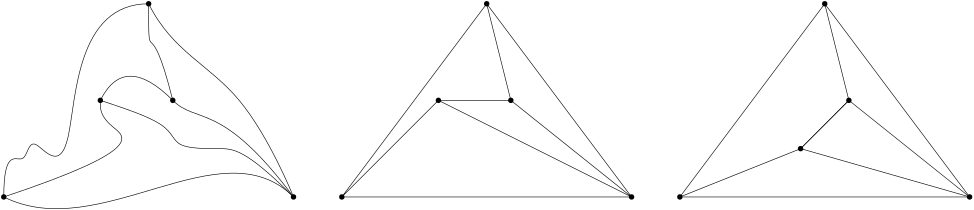
\includegraphics[width=0.9\textwidth]{topo_straight_convex.png}
	\caption{Planarer Graph mit einer topologischen, einer geradlinigen und einer konvexen Zeichnung.}
	\label{cut_figure}
\end{figure}

\begin{definition}[intern zusammenhängend]\label{int_3_con}
Ein Graph $G$ ist zusammenhängen falls für alle Knoten $u,v$ ein Pfad von $u$ nach $v$ exisitert. $G$ ist \textit{k-zusammenhängend}, falls er nach der Entfernung von $k-1$ beliebigen Knoten weiterhin zusammanhängend ist.\\
Sei $G$ plan mit den Aufhängungen $a_1,s_2,a_3$, weiter sei $a_\infty$ ein zusätzlicher Knoten im äusseren Gebiet. Dann ist $G$ \textit{intern k-zusammenhängend}, falls $G \cup \{ a_1a_\infty,a_2a_\infty,a_as_\infty \}$ k-zusammenhängend ist. 
\end{definition}

In den Siebzigern betrachtete William Thomas Tutte die Unterklasse der drei-zusammenhängenden planaren Graphen und zeigte, dass für diese nicht nur geradlinige, sondern sogar \textit{konvexe} Zeichnungen existieren, bei denen alle Gebiete die konvexe Polygone umranden. \cite{tutte63}
